\chapter{State-of-the-Art} \label{chap:State}

In the previous chapter, we introduced our project, including our project motivation and aims. In this chapter, we describe the current state-of-the-art in the research area where our project lies and discuss relevant technologies and concepts upon which the current project is built. In Section \ref{sec:SDN}, we discuss the concept of Software-Defined Networking, which is the fundamental building block of our project. Subsequently, in Section \ref{sec:HadoopTraffic}, we analyse and contrast studies that have used Software-Defined Networking to optimize Hadoop application traffic, on the basis of which, the current project is based. And finally, in Section \ref{sec:Emulators}, we describe emulators used for emulating data centre networks and Hadoop jobs respectively, which have made this project possible. 

\section{Software-Defined Networking} \label{sec:SDN}

Fast paced innovations in Computing have accelerated the growth and adoption of technology throughout the world in every sphere of life. However, innovations in Computer Networking have not been very steady, part of it was because of the unwillingness to conduct experiments in a network carrying production traffic. Moreover, there were a large number of protocols and network equipment already deployed in the network, which made it more difficult to innovate \cite{mckeown2008openflow}. 

Software-Defined Networking (SDN) enables controlling of the entire network through a centralized controller which maintains state of the entire network and is responsible for functions such as the routing protocols used by the forwarding devices in the network \cite{lantz2010network}. SDN achieves this by separating the control plane from the forwarding plane, where the control plane is housed in the centralized controller, and the forwarding plane is controlled via a narrow channel such as the OpenFlow protocol \cite{mckeown2008openflow}, as illustrated in Figure \ref{fig:OpenFlowOverview}. Communication between the OpenFlow switches and the centralized controller is achieved over a secure channel which is encrypted via SSL. 
\begin{figure}[!ht] 
	\centerline{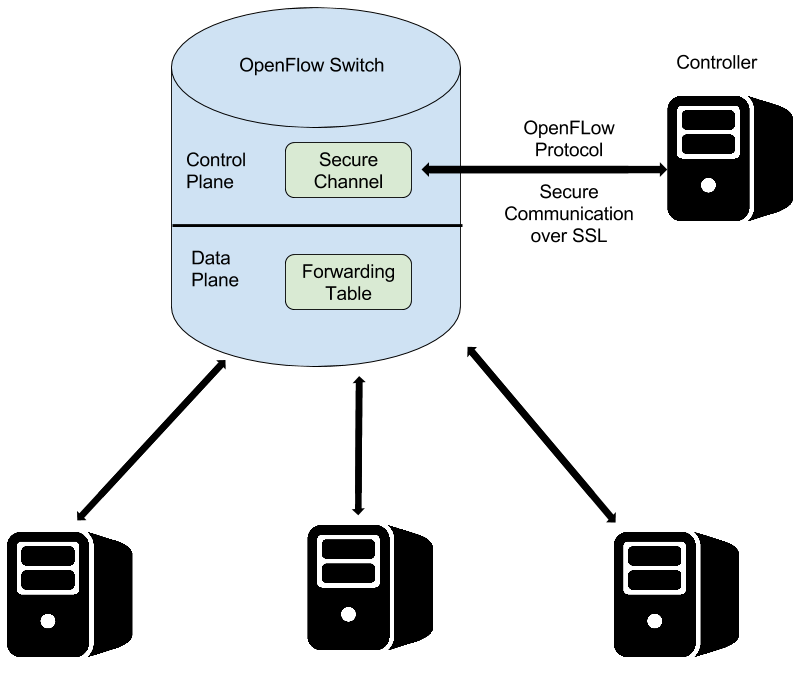
\includegraphics[scale=0.33]{graphics/chapter2/OpenFlowProtocol.png}}
	\caption{Overview of the operation of the OpenFlow protocol, where forwarding behaviour of switches is controlled by a centralized controller via a secure channel.}
	\label{fig:OpenFlowOverview} 
\end{figure}

Consequently, new functionality can be added in networks that are already deployed without any modification to the switches, and prototyping of new ideas can be conducted  without disrupting production traffic, enabling innovation in networking at software speeds \cite{lantz2010network}. 

SDN has resulted in a significant amount of research conducted with the aim of optimizing routing protocols and managing the network more efficiently \cite{kreutz2015software}. Examples of SDN Networks include FlowVisor \cite{sherwood2010carving}, PortLand \cite{niranjan2009portland} and Ethane \cite{casado2007ethane}. In this project, we leverage SDN to optimize data centre networks for Hadoop \cite{HadoopWeb} traffic. 
%\pagebreak
\section{Hadoop Traffic Optimization using SDN} \label{sec:HadoopTraffic}


\begin{table}[!ht]
\caption{Comparison of various studies that attempt to optimize data centre traffic of applications such as Hadoop using SDN} 
	\begingroup 
	\setlength{\tabcolsep}{5pt} % Default value: 6pt
	\renewcommand{\arraystretch}{1.2} % Default value: 1, use it to increase decrease padding
	\centerline{\begin{tabular}{|>{\columncolor[gray]{0.8}}L{2.2cm}|L{2.4cm}|L{2.4cm}|L{2.4cm}|L{2.4cm}|L{2.4cm}|} 
			\hline
			Study       & FlowComb \cite{das2013transparent} & Wang \textit{et al.} \cite{wang2012programming} & HybridTE \cite{wette2015hybridte} & Pythia \cite{neves2014pythia} & Hedera \cite{al2010hedera}  \\ \hline
			Approach    & Reactive & Reactive & Semi-Proactive & Reactive & Reactive \\ \hline
			Methodology & Software agents on every node report  demands, used to route traffic & Interface SDN controller with Hadoop master,which reports demands to controller & Install mice flows proactively and elephant flows reactively & Hadoop middleware predicts future transfers, network arranged accordingly  & Devised new flow scheduling algorithms as an extension to ECMP \\ \hline
			Uses Hadoop Traffic & Yes &  Yes & No & Yes & Yes \\ \hline 
			Result      & Reduced Hadoop Runtime by 33\% & Proposal, No Results & Outperforms Hedera and ECMP in flow completion times & Reduced Hadoop runtime by 43\% compared to ECMP & 39\% better bisection bandwidth achieved for Hadoop shuffle phase, compared to ECMP \\ \hline
			Limitations & Agents cause computational overhead, require domain specific knowledge & Requires creating demand estimator, computational overhead on master node & Underutilizes path diversity for mice flows, elephant flow detection suffer latencies & Domain-specific, intrusive to app data, induces computational overhead & 100ms latency in Scheduling due to control overhead, might increase when scaled to millions of hosts  \\ \hline 
			Type & Application-Aware & Application-Aware & Application-Aware & Application-Aware & Traffic-Aware  \\ \hline 
			\end{tabular}} 
		\endgroup
		\label{table:StudiesComparison}
\end{table}

In this section, we review various recent studies \cite{das2013transparent, wang2012programming, al2010hedera, narayan2012hadoop, neves2014pythia, wette2015hybridte} that have been conducted with the aim of optimizing application traffic of Big Data processing applications such as Hadoop \cite{HadoopWeb} (described in detail in \ref{subsec:HadoopOverview}), in a data centre network using SDN; in order to achieve faster data processing times through high network utilization. We give a high level overview and comparison of these studies in Table \ref{table:StudiesComparison}. Most of the work done in this area uses \textit{reactive} measures for data centre network configuration, which motivated us to explore a \textit{proactive} approach, as described in Chapter \ref{chap:design}. 

All the studies compared in Table \ref{table:StudiesComparison} employ \textit{multi-rooted} tree topologies, which are described in detail in \ref{sec: DataCentreArch}, while they compare their performance against Equal Cost Multi-Path (ECMP) \cite{hopps2000analysis} routing, which is the industry standard protocol for routing traffic in a multi-rooted tree topology having path diversity. ECMP is described in detail in \ref{subsec:ECMP}. All approaches to optimize Hadoop traffic using SDN can be broadly classified into \textit{Application-Aware networking} and \textit{Traffic-Aware Networking}. Studies employing the two approaches are discussed in the next subsections.

\subsection{Application-Aware Network Optimization} \label{subsec:AppAware}

\begin{figure}[!ht] 
	\centerline{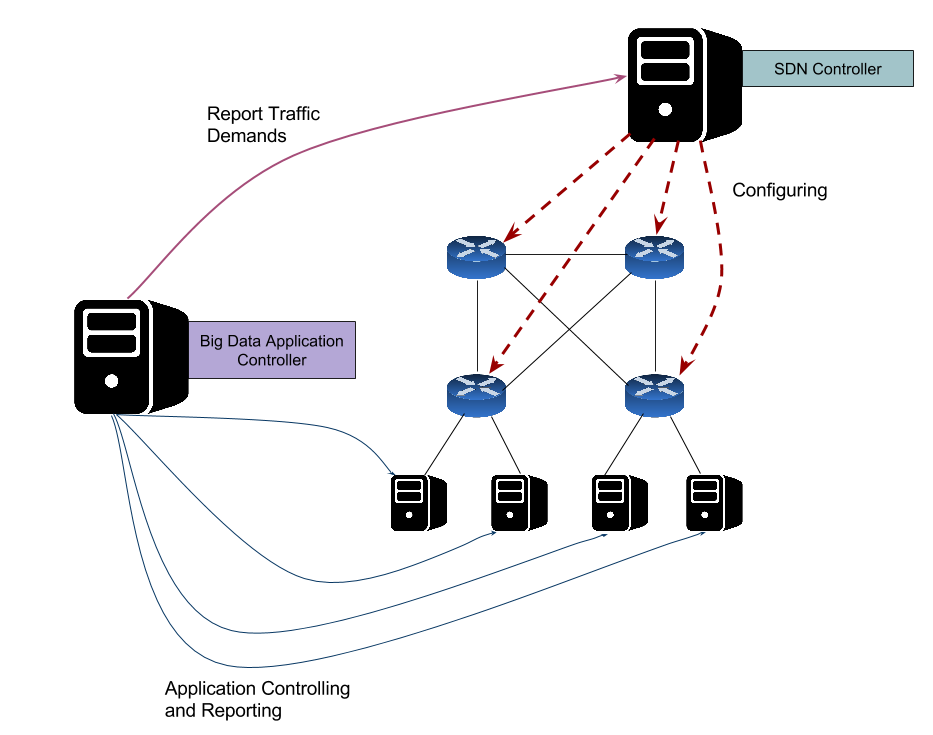
\includegraphics[scale=0.40]{graphics/chapter2/ApplicationAwareScheduling.png}}
	\caption{The big data application controller reports traffic demands to the network controller, enabling \textit{Application-Aware} flow scheduling.}
	\label{fig:ApplicationAwareScheduling}
\end{figure}

Figure \ref{fig:ApplicationAwareScheduling} illustrates the approach of \textit{Application-Aware} scheduling in order to optimize the network for Big Data applications. It attempts to tightly integrate Big Data application controllers with the SDN controller responsible for scheduling of flows in the network. The application controller reports traffic demands to the SDN controller on the bases of information obtained from the hosts, which is used by the SDN controller to configure forwarding devices in the network in a \textit{reactive} manner. We further discuss this approach of network optimization by analysing studies that are based on this methodology for network optimization.
 
Das \textit{et al.} \cite{das2013transparent} attempted to optimize Hadoop by introducing a network management framework called \textit{FlowComb} that leverages SDN and monitoring of all servers running Hadoop, to perform dynamic scheduling of flows.  

The main objectives of \textit{FlowComb} were to predict the network demand of an application in advance and dynamically install flows in the network switches based on its prediction. Das \textit{et al.} argued that studies monitoring the network to detect changes such as \textit{Hedera} \cite{al2010hedera}, do so only after a change has occurred; moreover network monitoring is an expensive operation. In order to anticipate network demands, Das \textit{et al.} developed software agents which were installed on all servers running Hadoop in a cluster. The Software agents essentially performed two functions, namely, scanning Hadoop logs to extract information about map tasks and network transfers; and sending this information to the scheduling component of \textit{FlowComb}, which is the SDN controller, thereby making the SDN controller \textit{application-aware}. 

Similar to Hedera \cite{al2010hedera} as described in \ref{subsec:Hedera}, \textit{FlowComb's} Scheduling engine dynamically allocates and installs paths in the network using the OpenFlow protocol \cite{mckeown2008openflow}; in order to avoid traffic congestion and provide sufficient bandwidth to all flows. \textit{FlowComb} was found to reduce the average running time of sorting 10 GB of data in a 14 node Hadoop cluster by \textit{33\%} \cite{das2013transparent}. 

\textit{FlowComb} has a number of drawbacks, such as it depends on domain-specific knowledge to operate, hence the same implementation of \textit{FlowComb} cannot be applied to different MapReduce implementations apart from Hadoop \cite{HadoopWeb}, such as Dryad \cite{isard2007dryad} and Spark \cite{SparkWeb}. Furthermore, since reducers start transfers at random, \textit{FlowComb} cannot determine the exact timing of the start of a transfer \cite{das2013transparent}; extracting information at the hosts by scanning Hadoop logs causes a computation overhead and finally, \textit{FlowComb} helps in optimizing Hadoop jobs only when the network is congested. 

Similarly, Wang \textit{et al.} \cite{wang2012programming} have proposed to tightly integrate Big Data applications with network control by leveraging the programmability of networks provided by SDN and the high network bandwidth provided by optically switched networks, making the network \textit{application-aware}. Since applications such as Hadoop \cite{HadoopWeb} have a master node that maintains an overall control over the other nodes in a cluster, as described in \ref{subsec:HadoopOverview}, Wang \textit{et al.} suggest to interface the SDN controller with the master node, thereby enabling application controllers to report traffic demands to the SDN controller and issue topology configuration commands to the SDN controller, on the basis of which, the network is configured \textit{reactively}.

The approach suggested by Wang \textit{et al.} \cite{wang2012programming} would have to overcome a number of challenges. A demand estimator engine would need to be implemented for every application that has to be interfaced with the SDN controller for the master node, which would introduce a significant computational overhead for the master node \cite{wang2012programming}. The \textit{reactive} nature of configuring the topology at runtime, as suggested by Wang \textit{et al.} imposes significant computational responsibilities on the SDN controller to re-configure the network in response to traffic demands with low latency, and imposes a challenge on the SDN controller's scalability.

Wette \textit{et al.} \cite{wette2015hybridte} argue that \textit{reactive} approaches such as Hedera \cite{al2010hedera}, which try to optimize data centre networks by reactively installing flow entries, overwhelm the switching hardware by the number of flows that they tend to install. In order to alleviate overwhelming of switching hardware, Wette \textit{et al.} propose a \textit{semi-proactive} approach of flow scheduling called \textit{HybridTE}. By exploiting explicit knowledge about elephant flows, \textit{HybridTE} is able to perform flow scheduling using very few flow entries in the switches. \textit{HybridTE} treats mice flows and elephant flows differently, by installing flow entries \textit{proactively} for mice flows  and \textit{reactively} for elephant flows. 

Using a data centre architecture as described in \ref{sec: DataCentreArch}, \textit{HybridTE} installs one forwarding tree per ToR switches using OpenFlow wild-card flow table entries in a \textit{proactive} manner, which, Wette \textit{et al.} argue is sufficient for small flows. As far as the elephant flows are concerned, Wette \textit{et al.} investigate the effect of different techniques for elephant flow detection such as HadoopWatch \cite{peng2014hadoopwatch}, which monitor Hadoop logs to predict upcoming file transfers and packet sampling, which has been demonstrated by Choi \textit{et al.} \cite{choi2004adaptive} to be effective in determining elephant flows when using a reasonable sample. Using elephant flow detection schemes as previously described, \textit{HybridTE} re-routes elephant flows to the shortest path which is the least congested, in a \textit{reactive} manner. 

\textit{HybridTE} was found to outperform ECMP \cite{hopps2000analysis} and Hedera \cite{al2010hedera} in terms of flow completion times, with ECMP taking 29.1\% longer times for flow completion in a network with increasing congestion than \textit{HybridTE} \cite{wette2015hybridte}. However, \textit{HybridTE} has certain limitations such as it does not exploit path diversity for routing mice flows, and detecting elephant flows to avoid congestion has inherent high-level latencies.  

\textit{Pythia} \cite{neves2014pythia} is another study that aims to optimize Hadoop job completion times by predicting Hadoop data transfers at runtime and avoiding congestion during the Hadoop shuffle phase by dynamically routing network flows. \textit{Pythia} has two components

\begin{itemize}
	\item Hadoop instrumentation middle-ware that runs on all of the Hadoop worker nodes, responsible for predicting future shuffle transfers by extracting information from Hadoop logs, similar to software agents employed by FlowComb \cite{das2013transparent}.
	\item An Orchestration entity that dynamically allocates reactive paths on runtime on the basis of future shuffle transfers predicted by the middle-ware which is sent to it. 
\end{itemize} 

The Hadoop instrumentation middle-ware is able to determine the size of a data transfer, since after a map task finishes, it writes the intermediate $<$key, value$>$ pairs to disk \cite{narayan2012hadoop}, which is read by the instrumentation middle-ware \cite{neves2014pythia}. The size of the future transfer, along with the map task ID is subsequently transmitted to the orchestration controller, which \textit{reactively} configures the network based on the supplied prediction.  

Neves \textit{et al.} evaluated \textit{Pythia} on a cluster of 10 servers with a total RAM of 128GB and found that \textit{Pythia} outperforms ECMP which is the industry standard for multipath routing, as explained in \ref{subsec:ECMP}; by lowering Hadoop job completion times by 43\% \cite{neves2014pythia}. However, \textit{Pythia} has certain limitations, such as the Hadoop instrumentation layer is able to access Hadoop logs, making it intrusive and difficult to implement in a multi-tenant data centre, with different Hadoop jobs running simultaneously causing a computational overhead at the worker nodes. \textit{Pythia} is very specific to Hadoop and would not function for a broader range of communication patterns. 

\subsection{Traffic-Aware Network Optimization}

In contrast to \textit{application-aware} network optimization, as discussed in \ref{subsec:AppAware}, \textit{traffic-aware} network optimization seeks to optimize the network by continuously monitoring forwarding devices and reporting the changing traffic information to the SDN controller, as illustrated in Figure \ref{fig:TrafficAwareScheduling}, which subsequently performs flow scheduling on the bases of the reported information. This monitoring can be done via the SDN controller itself, since it can request traffic statistics from OpenFlow switches. 

\begin{figure}[!ht] 
	\centerline{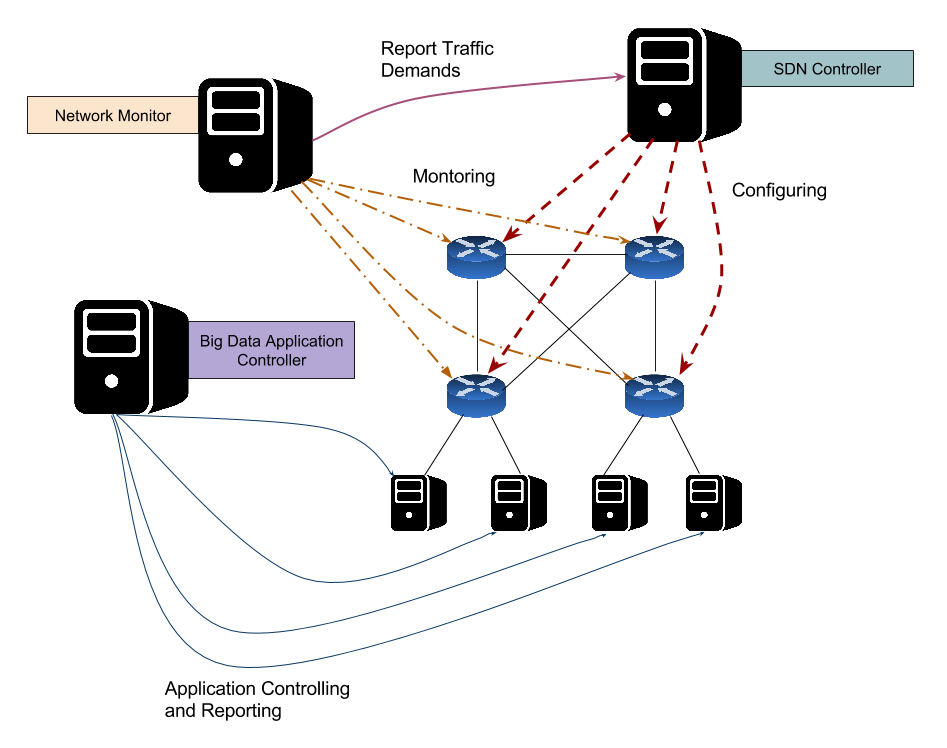
\includegraphics[scale=0.40]{graphics/chapter2/TrafficAwareScheduling.png}}
	\caption{The network is monitored continuously to keep track of traffic demands, enabling \textit{Traffic-Aware Scheduling}.}
	\label{fig:TrafficAwareScheduling}
\end{figure}

\textit{Hedera} \cite{al2010hedera} is one such study that employs \textit{traffic-aware} scheduling. The study proposes an extension to ECMP, whereby, it routes flows exceeding a certain threshold in a \textit{reactive} manner. We do a more comprehensive discussion on Hedera's Global First-Fit flow scheduling algorithm in \ref{subsec:Hedera} and evaluate implementations of ECMP and Global First-Fit against our \textit{proactive} approach in Chapter \ref{chap:eval}. \textit{Hedera} was found to significantly reduce Hadoop shuffle transfer times in comparison to ECMP routing, achieving 39\% more of the total bisection bandwidth available in the network, as compared to ECMP.

\section{Emulators for Data Centre Experimentation} \label{sec:Emulators}

In this section, we describe the emulators that we used for the implementation of our current project, detailed in Chapter \ref{chap:Implmentation}, since we did not have access to a cluster of servers for running our experiments. Firstly, in \ref{subsec:DataCentreEmulation}, we describe the emulator used for emulating data centre networks and subsequently, in \ref{subsec:Mremu} we describe an emulator that emulates the working of Hadoop \cite{HadoopWeb} using real Hadoop traces.  

\subsection{Data centre Network Emulation}  \label{subsec:DataCentreEmulation}
In order to exploit the full potential of SDN as described in \ref{sec:SDN}, it should be possible to prototype novel approaches for network control without the need of running experiments in a data centre, since all researchers do not have access to such resources. Lantz \textit{et al.} \cite{lantz2010network} filled this gap by introducing \textit{Mininet}, which is a lightweight virtualization platform for prototyping SDN Networks. \textit{Mininet} can work on the constraint resources of a single laptop. It is built with the following attributes
\begin{itemize}
	\item Allows defining of new topologies and functionality using familiar programming languages, specifically, python \cite{van2007python}.
	\item Network can be deployed from virtual to physical hardware without any change in code, with high degree of fidelity in behaviour. 
	\item Allows managing the network in real time, scaling to thousands of switches on a single physical host. 
\end{itemize} 

Code created in other similar emulators like Opnet \cite{opnetWeb} and ns-2 \cite{ns2} for network simulation cannot be ported directly to real hardware; moreover, they don't provide the functionality of interacting with the network in real time \cite{lantz2010network}. On the other hand, \textit{Mininet} leverages Linux features such as network namespaces and virtual Ethernet pairs, enabling it to offer support for networks with bandwidth in Gigabits and hundreds of nodes such as controllers, switches and hosts; all of which are emulated with ease on a single laptop. All these attributes made \textit{Mininet} the ideal choice of network emulator for our current project since we did not have access to a cluster of servers.

\textit{Mininet} combines its lightweight Linux virtualization with an interactive command line interface and an extensible API written in python to experiment with SDN. The interactive CLI can be used to manage the entire SDN network from a single command line while a simulation is running. The \textit{Mininet} python API can be used to define custom network topologies, node types and experiments \cite{lantz2010network}.

\textit{Mininet} uses Open vSwitch \cite{OpenvSwitch} for emulating OpenFlow switches in the network, and works well with all SDN controllers such as POX/NOX \cite{gude2008nox}, OpenDayLight \cite{ODL2016}, \textit{et cetera}. A \textit{Mininet} host is essentially a shell process which resides in it's own namespace \cite{lantz2010network}, having virtual Ethernet interfaces,  making it very lightweight. An SDN controller can work with \textit{Mininet} as long as the switches running in mininet have IP connectivity to the controller \cite{lantz2010network}.

\textit{Mininet} scales well to over 1000 nodes owing to sharing of the file system, process ID space, kernel and other resources, providing a bandwidth of 1-3 Gbps through a single switch \cite{lantz2010network}, making it ideal for running emulations of a data centre network on a single laptop. However, \textit{Mininet} has certain limitations, such as it suffers from a lack of performance fidelity when the emulation has high loads, additionally, software based forwarding cannot surpass the speeds obtained by TCAM accelerated vendor switches, live host migration is not supported and \textit{Mininet} does not support distributed emulation since it can only run on a single machine. Nonetheless, \textit{Mininet} offers a viable alternative to running experiments in real hardware and provides a scalable and interactive environment with an extensible API to conduct experiments, which is why we chose it for implementing our experiment as described in Chapter \ref{chap:Implmentation}.  


\subsection{Hadoop Emulation} \label{subsec:Mremu}

Use of real hardware robust enough for running data centre experiments is not a valid option for many researchers since such resources are not readily available. We faced a similar problem, therefore we chose to run the experiments of this project on a Hadoop emulator-based test bed.   

The emulator that met our requirements was MRemu, devised by Neves \textit{et al.} \cite{neves2015mremu}. MRemu is a framework that works as a Hadoop emulator by reproducing traffic patterns of a Hadoop job trace with the same latencies as in the original Hadoop job trace. Hence, using MRemu, Hadoop jobs are emulated in hosts running on Linux containers \cite{neves2015mremu} such as \textit{Mininet}, as described in \ref{subsec:DataCentreEmulation} to emulate data centre nodes, running on a single physical host, which have low IO and CPU resources to run a real Hadoop job.

Studies have demonstrated that MapReduce applications are sensitive to performance of the network \cite{das2013transparent, chowdhury2011managing}, nonetheless, numerous studies use synthetic traffic patterns, generated following certain probabilistic distributions \cite{al2008scalable, greenberg2009vl2, curtis2011devoflow}, which fails to capture the true network workloads \cite{neves2015mremu}. Taking this into consideration, Neves \textit{et al.} developed a tool for extracting traces from Hadoop job execution logs with enriched network information to generate comprehensive Hadoop job traces to be used with MRemu. These traces \cite{MRemuRepo2015} produced by Neves \textit{et al.}, made available online, have been employed by us in this project. 

\begin{figure}[!ht] 
\centerline{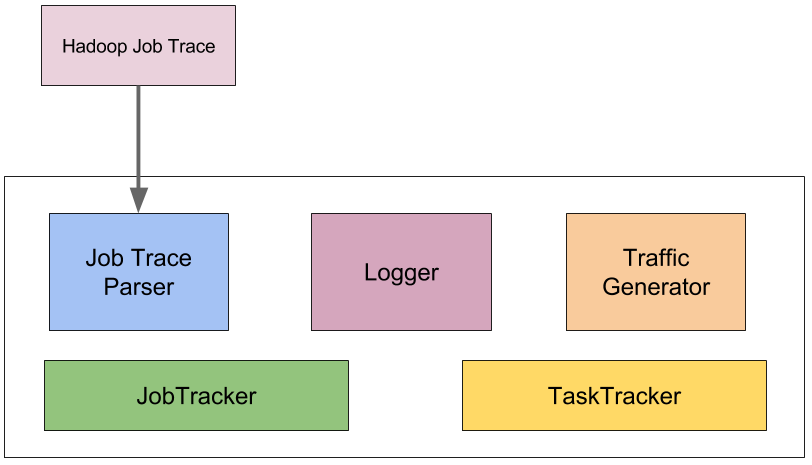
\includegraphics[scale=0.30]{MRemuOverview.png}}
\caption{Block Diagram of MRemu Hadoop Emulator.}
\label{fig:MRemuOverview}
\end{figure}

Figure \ref{fig:MRemuOverview} shows a high level overview of the Hadoop emulator in MRemu. Hadoop job traces are fed to the Job Trace parser, which uses information from the trace, such as wait times and task durations, to mimic the latencies in a real Hadoop job execution. The traffic generator generates \textit{iperf} flows, mimicking network transfers of the real Hadoop job corresponding to the trace, while the logger logs Hadoop events to local disk of the emulated nodes.  

MRemu makes it possible to test different network routing control logic using SDN for Hadoop traffic on the constraints of a single physical system, making it ideal to be used in conjugation with \textit{Mininet}, as described in \ref{subsec:DataCentreEmulation}, for Hadoop traffic scheduling experimentation. MRemu supports production SDN controllers such as POX/NOX \cite{gude2008nox} and OpenDayLight \cite{ODL2016}, making it ideal for evaluating novel approaches to route Hadoop traffic in order to accelerate it. 

Neves \textit{et al.}  \cite{neves2015mremu} tested MRemu, by first obtaining Hadoop traces from a real cluster of 16 identical nodes, running Hadoop 1.1.2, while the emulation was performed on a single node with 16 GB of RAM and 16 x86 64 cores, running on \textit{Mininet} 2.1.0. The original Hadoop jobs ran applications forming part of the HiBench Benchmark Suite \cite{huang2011hibench} such as Bayes, Sort, Nutch and PageRank. On performing a comparison between job completion times in real hardware and the MRemu emulation setup, Neves \textit{et al.} observed that the job completion times were comparable. Furthermore, Neves \textit{et al.} evaluated individual flow completion times as well and found the transfer durations in the emulation to be slightly different than the real transfer durations, owing to inaccuracies in Hadoop logs (used to extract traces) due to high-level latencies. Nonetheless, Job Completion times were found to be near accurate, owing to which, we chose to use MRemu for evaluating our proactive approach as described in Section \ref{chap:Implmentation}. 

However, MRemu has certain limitations, such as 

\begin{itemize}
\item MRemu supports emulation of only one job at a time, having no support of concurrent job execution. 
\item MRemu does not model failure handling techniques of Hadoop, making it a requirement of only running successful job traces for emulation \cite{neves2015mremu}.
\item MRemu does not support distributed emulation, hence it can only support a limited number of Linux container nodes that can be supported by a single physical server and cannot scale to hundreds of nodes. 
\end{itemize}

Nonetheless, MRemu adequately met our requirements for a Hadoop emulator that can be run over \textit{Mininet}, therefore, we chose to use it for the current project in conjugation with \textit{Mininet}.
 

